\section{Communication}%{{{
\label{sec:communication}

\subsection{L'affiche}%{{{
\label{sub:l_affiche}

La communication étant importante pour la réalisation du projet, nous sommes partis sur l'élaboration
d'une affiche A3.

Nous avons souhaité que cette affiche se devait d’être contrastée et peu chargée afin qu’elle soit
claire et lisible de loin, c’est pourquoi la combinaison du noir sur fond blanc fut adaptée à ce choix.
De plus, il fallait que l’identité visuelle de l’affiche puisse parler aux joueurs, d’où l’utilisation
d’une police spéciale de grande taille, police de la licence \og Starcraft \fg{}, et placée en haut de l’affiche.

La date et le lieu bénéficient également d’une taille plus grande que le texte du corps de l’affiche.
Concernant ce dernier, nous avons décidé de ne pas le charger en texte afin de bénéficier d’une police
plus grande grâce à l’espace obtenu.
Nous avons mis en avant la venue du commentateur et joueur Soey de niveau \og top master \fg{} dans le but
de donner une plus grande crédibilité à l’évènement.
Enfin, pour rajouter à l’identité visuelle, nous avons fait figurer les emblèmes des trois races du jeu,
ainsi qu’une grande bannière où apparaît le protagoniste principal de la prochaine extension.
21 affiches ont été imprimées au format A3, pour ensuite être affichées dès le 1er mars à l’IUT A, au M1,
au M3, au M5, à la MDE et dans quelques résidences universitaires.

% subsection l_affiche (end)%}}}
\subsection{L'enquête d'audience}%{{{
\label{sub:l_enquete_d_audience}

L'affiche seule n'étant pas suffisante pour la communication, nous nous sommes tournés vers la
Maison Des Étudiants et son e-mail afin de diffuser l'information à tous les étudiants de l'université.
Profitant de ce moyen, nous avons élaboré un questionnaire. Le but de celui-ci était d'obtenir une estimation
du nombre de participants et trouver un potentiel commentateur.

Malheureusement, le mail n'a été envoyé que le 5 mars, soit une semaine avant l'évènement.
Nous avions néanmoins déjà trouvé notre commentateur.

L'enquête est un questionnaire comporte quatre à neuf questions selon
les réponses des sondés. 30 ont répondu.  Vous pouvez consulter les
graphiques générés de ces questions sur les figures \ref{char1},
\ref{char2} et \ref{char3} en page \pageref{char1}.

\begin{figure}
  \begin{center}
    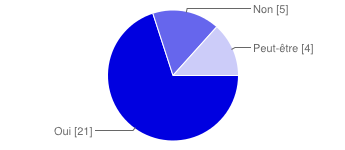
\includegraphics[scale=1]{images/chart_1.png}
    \caption{Êtes-vous intéressé par une soirée Starcraft 2 (WoL, HotS) ?}
    \label{char1}
  \end{center}
\end{figure}

\begin{figure}
  \begin{center}
    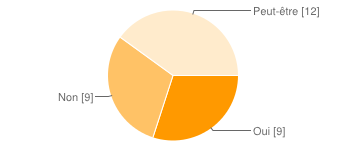
\includegraphics[scale=1]{images/chart_2.png}
    \caption{La soirée se déroulera un mercredi soir (18h-23h), serez-vous présent ?}
    \label{char2}
  \end{center}
\end{figure}

\begin{figure}
  \begin{center}
    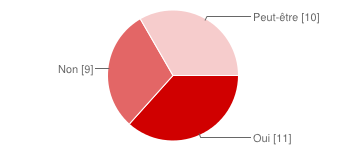
\includegraphics[scale=1]{images/chart_3.png}
    \caption{Aimeriez-vous y jouer au cours de cette soirée ?}
    \label{char3}
  \end{center}
\end{figure}

Nous pouvons tirer de ces informations une estimation de plus ou moins 15 personnes présentes si l’on prend
la moitié des \og peut-être \fg{} additionné au \og oui \fg{}.
En sachant que tous les étudiants ne prêtent pas attention aux mailings de l’université, on peut ajouter
une quinzaine de personnes pour atteindre une estimation de 30 participants.

% subsection l_enquete_d_audience (end)%}}}
\newpage
\subsection{Les contraintes/ratés}%{{{
\label{sub:les_contraintes_rates}

Un autre moyen de communication fut utilisé, la création d'un évènement
Facebook. Néanmoins cela n'a pas fonctionné, la propagation de cet
évènement ne fut pas suffisante sur le réseau social. De plus cette page
de promotion a été ouverte très tardivement ce qui fait que nous
n'avons pas eu le temps de faire marcher les connaissances.

La contrainte majeure concernant l'élaboration de la communication fut l'attente
de la confirmation de tous les éléments du projet. Nous ne pouvions
notamment pas lancer la production des affiches sans savoir si nous
avions un commentateur par exemple.

% subsection les_contraintes_rates (end)%}}}

% section communication (end)%}}}
